\documentclass{scrartcl}

\usepackage{Header}

%\usepackage{scalefnt}
%\usepackage{parcolumns}
%\usepackage{tikz-er2}
\usepackage{hyperref}

\begin{document}


\Gruppe{Stephan Heidinger}{DBS - Zusammenfassung, V 0.3a}
\Header{Datenbanken und Informationssysteme}{Sommersemester 2011}{Stephan Heidinger}{}%leave last variable empty, else there will be aufgabenblatt überschrift

\begin{shaded}
Dieses Dokument wurde unter der Creative Commons - Namensnennung-NichtKommerziell-Weitergabe unter gleichen Bedingungen (\textbf{CC by-nc-sa}) veröffentlicht. Die Bedingungen finden sich unter \href{http://creativecommons.org/licenses/by-nc-sa/3.0/de}{diesem Link}. \\
\centerline{
\includegraphics[scale=1]{../cc-by-nc-sa.png} }
\end{shaded}

\textit{Find any errors? Please send them back, I want to keep them!}

\section*{Abstraction}
\begin{itemize}
	\item Three kinds of data abstraction: External schema $\to$ Conceptual schema  $\to$ Internal Schema  $\to$ Stored Data
	\item \textbf{Conceptual Schema:} simplified view of DB, modeling abstractions, semantic constraints.
	\item \textbf{Internal/Physical Schema:} \textit{(Implementation)} Indexing, Division of tables among disks, storage management, Placement of new rows in tables
	\item[Abstraction:] applications dont care about how it works exactly, as they can access the db in the same way.
	\item[Abstraction:] later modification of db (addition of information) should not lead to modification of apps
	\item \textbf{External Schema/View:} subset of whole db, security reasons, need-to-know
\end{itemize}

\section*{State vs Schema}
\begin{itemize}
	\item \textbf{Database Schema:} formal definition of the structure of dbs contents, defined, when db is created
	\item \textbf{Database State:} \textit{(Instance of the Schema)} Contains actual data, changes frequently
	\item data is structured in tables (relations) with name, namend columns (attributes) and set of rows (tuples)
	\item db queries refer to conceptual schema, dbms translates into execution plan that refers to internal schema, optimizes (more complex queries $\Rightarrow$ bigger savings)
	\item \textbf{declarative query languages:} describe what information is sought, not how ($\Rightarrow$ \textsc{SQL})
\end{itemize}

\section*{Transaction Management}
\begin{itemize}
	\item \textit{virtual machine illusion}, isolation of concurrency, fault tolerance, atomic commit, consistency checking, distributed coordination
	\item[ACID:] \textit{(atomicity, consistency, isolation, durability)} sequences of db commands are executed as \textbf{atomice unit}, support for backup an recovery, support for concurrent users
\end{itemize}

\section*{Database Management System (DBMS)}
\begin{itemize}
	\item generic, application independent software system implementing a data model
	\item definition of DB schema, storage of an instance of this schema, querying the instance, changing the state, defining users and privilieges
	\item \textbf{Data Model:} formal languages: DDL \textit{(data definition language, declaring database schema)}, (S)QL \textit{(querying the current database state)}, DML \textit{(database manipulation language, changing the state)}
	\item[i.e.:] Relational Model, Entity Relationship Model, Object-Oriented Models, UML, XML
	\item application programs process users request, formulate sql statements, present the result in a user-friendly way
	\item \textbf{DB applications Systems:} users access database concurrently, dbms runs as background server processes,
	\item \textbf{Database users:}
	\begin{description}
		\item[Database Administrator (DBA):] know about all schemas, change conceptual and internal schema, gives acces rights to users, security, monitors performance/disk space/etc, backups, recoveries
		\item[Application Programmer:] writes programs for use by na"ive users (safe data entry, report generation, data browsing), knows sql/programming languages well, supervised by DBA, might do conceptual design
		\item[sophisticated User:] knows something of sql, may use SQL-console/generic db-tools, non-standart aggregations/evaluations w/o help from programmers
		\item[na"ive user:] uses db only via applictaion programs, often unaware of db itself, data entry, browsing, external views
	\end{description}
	\item \textbf{Database tools:}(interactive) sql console, graphical/menu-based query-tools, interface for db-access for standart programming languages, report generators, web interface, import/export/backup/recovery/performance monitoring/... tools
\end{itemize}

\section*{Information Modelling}
\textit{...the process of revising a (formal) model of (parts of) the real world.}
\begin{itemize}
	\item ...Herauslassen von details, Konzentrieren auf die "`wichtigen"' Sachen
	\item meist "`Bilder anstatt Sprache"'
\end{itemize}

\section*{Relational Model \& SQL Introduction}
\begin{itemize}
	\item  database $\to$ set of tables; schema defines: names of tables, columns of each table, integrity constraints
	\item Table $\equiv$ relation,  Row $\equiv$ tuple, Column $\equiv$ attribute, Data type of column $\equiv$ domain of attribute, Table entry $\equiv$ attribute value
	\item \textbf{key:} always identifies a single row in a table (keys are contraints)
	\item \textbf{foreign key:} no physical pointer in relational model, foreign keys "`point"' to other tables, foreign key and reference may have different names
	\item \textbf{bad relational tables:} redundancy, many empty cells, several real world concepts in one table
	\item \textbf{SQL:} \textsc{Select} \texttt{<attr>} \textsc{From} \texttt{<table>} \textsc{Where} \texttt{<condition>} \\ SQL ist case-insensitive, außer in strings, wildcards (use \textsc{Like)}: \% - sequence, \_ single character, remove duplicates: \textsc{Distinct}, sorting: \textsc{Order By [Asc|Desc]}
\end{itemize}

\section*{Entity-Relational Model}
\begin{itemize}
	\item \textbf{DB design hard:} Expertise (designer has to know the field he is designing or needs an expert, which may be a \textsc{Wdg}), Flexibility (exceptions, corner cases, ...), Size \\ $\Rightarrow$ DB design as a \emph{multi-step} process.
	\item \textbf{Three Phases of DB Design:} (partitioning the problem, attack one problem after another, DBMS does not influence conceptual design, can change DBMS later on
	\begin{description}
		\item[Conceptual Database Design:] Produces initial model (conceptual data model, ER model)
		\item[Logical Database Design:] transform conceptual model into DBMS-conform model (relational model)
		\item[Physical Database Design:] indexes, table distribution, buffer size, etc $\to$ maximize performance
	\end{description}
	\item \textbf{ER Diagrams:} concept for easy design, good for communication with non-experts
	\begin{description}
		\item[Entity:] an object in the real world, must be distinguishable from each other (identity)
		\item[Relationship:] between pairs of entities
		\item[Attribute:] property or feature of an entity/relationship, the \textbf{value} is a data type (printable representation)
		\item[entity type:] set of similar entities
		\item[relationship type:] set of similar relationships
		\item[Cardinality:]$E_1$ is related to min $m_1$, max $n_1$ items of  $E_2$, * means no limit, weaker cardinalities: $(a,b) \textrm{ weaker than } (c,d) \Leftrightarrow a \leq c \land b\leq d$
	\end{description} 
	\begin{tikzpicture}[node distance=8em]
		\node[entity] (person) {E$_1$};
		\node[relationship] (commenting) [right of = person] {R} edge node[auto,swap] {($m_1,n_1$)}  (person);
		\node[entity] (photo) [right of = commenting] {E$_2$} edge node[auto,swap] {($m_2,n_2$)} (commenting);
		\node[attribute] (comment) [right of = photo] {A} edge (photo);
	\end{tikzpicture}
	\item \textbf{relationship between entities of the same type}: edges need role names (i.e. precondition and knowledge of)\\
	\begin{tikzpicture}[node distance=10.5em]
\node[relationship] (parent) {R};
\node[entity] (person) [right of = parent] {E};
\draw (person.165) edge [<-] node[auto,swap] {role1} (parent.35)
	(person.-165) edge node[auto,swap] {role2} (parent.-35);
\end{tikzpicture}
	\item \textbf{cardinalities:}
	\begin{description}
		\item[many-to-many:] $\square-(0,*)-\diamondsuit-(0,*)-\square$ or $\square-N-\diamondsuit-M-\square$: requires an extra table
		\item[one-to-many:] $\square-(\_,\blau{*})-\diamondsuit-(\_,\gruen{1})-\square$ or $\square-\gruen{1}-\diamondsuit-\blau{N}-\square$: \underline{do not require} an extra table
		\item[one-to-one:] $\square-(\_,1)-\diamondsuit-(\_,1)-\square$ or $\square-1-\diamondsuit-1-\square$
	\end{description}
	\item \textbf{key:} uniquely identifies the entity/relationship, composite keys allowed, keys not required in er, but required in relational schema, add artificial identifiers (ie numbers)
	\item \textbf{weak entitiey:} \textit{detail} entities that cannot exist without a \textit{master}/owner, cardinality (1,1) on detail side, key of master is inherited, keys always composite, inherited part of key not shown \\
\begin{tikzpicture}[node distance=8em]
\node[entity] (mother) {Mother};
\node[ident relationship] (has) [right of = mother] {has} edge [<-] node[auto,swap] {(0,1)} (mother);
\node[weak entity] (child) [right of = has] {Child} edge node[auto,swap] {(1,1)} (has);
\node[attribute] (motherID) [left of = mother] {\underline{Mother\_ID}} edge (mother);
\node[attribute] (childName) [right of = child] {\underline{Name}} edge node[auto,swap] { }(child);
\end{tikzpicture}
	\item \textbf{n-ary relationship:} relationships may connect more than 2 entities
	\item \textbf{association entity:} turns n-ary relationships into weak entities with multiple owners
	\item \textbf{supertype/Generalisation:} (i.e. mechanic is an employee) $\to$ child inherits attributes of parent, not shown in ER though
	\item \textbf{translation into realtional model:}
	\begin{itemize}
		\item create \textbf{table} for each entity
		\item \textbf{columns} are attributes
		\item \textbf{primary key} of the table is primary key of entity, if none available, add artificial key
		\item \textbf{weak entities}: 1table with key of owner are foreign keys
		\item \textbf{one-to-many:} key of "`one"' side added as foreign key into "`many"' table, minimum value shows, if null values are allowed or not
		\item \textbf{many-to-many:} create new table, keys of both entities, foreign composite primary key
		\item \textbf{one-to-one:} proceed like one-to-many, add key, where it makes more sense (i.e. null values can be enforced), no null values needed on both sides: one may have the attribute or extra table, if no null values on both sides $(1,1)-(1,1)$: merge tables
		\item \textbf{supertype/Generalisation:}
		\begin{enumerate}
			\item each entity type is mapped into seperate relation, superkey is foreign primary, each table holds only specific attributes, access requires joins, minimum redundancy
			\item one relation for all types, lots of \textsc{Null} values, additional distinguishing attributes (i.e. jobkind) may be needed, no joins
			\item independent relations for subtypes, generalisation lost, redundancy in schemas, redundancy in tuples, supertype relation needed
		\end{enumerate}
	\end{itemize}
\end{itemize}

\section*{beyond ER and relational modelling}
\begin{itemize}
	\item \grau{\textbf{object-orientation:}\\
	attributes $\to$ \textit{visibile internal structure} of entity (so ER does not provide encapsulation) or \textit{observer method} (so ER does provide encapsulation\\
	mutator $\to$ cannot be expressed in ER models (in SQL-3 possible) \\
	Aggregation (hirarchy) $\to$ "`part of"' relationships \\
	Association (hirarchy) $\to$ "`member of"' relationship}
	\item \grau{\textbf{UML:} (Unified Modeling Language) mostly graphical, "industry standard"' for language independent: analysis of requirements, visualisation of problems, design of programs/databases, communication with application/domain experts, implemenentation, documentation \\
	class: defines properties (attributes) and behaviour (methods), contains classname, attribute definition, method definition\\
	cardinalities: a,b  $\to$ exactly a or b, a..b  $\to$ between and including a and b, a..*  $\to$ at least a (or combinations)}
\end{itemize}

\section*{Relational Normal Forms}
\begin{description}
	\item[functional dependencies (FD)] generalisation of keys, things that depend on the key, form: $A_1,\dots,A_n\to B_1,\dots,B_m$ 
	\item[cover $\alpha^+$:] "`a set of attributes $\alpha$ is the set of all attributes $B$ that are uniquely determined by the attributes $\alpha$ (with respect to a given FD set $\mathcal{F}$): \[ \alpha^+_\mathcal{F} := \{ B \vert \mathcal{F} \textrm{ implies } \alpha \to B\} \]
	\textbf{Algorithm:}\\
$x \leftarrow \alpha ;$\\
$\texttt{while } x \text{ did change } \texttt{ do}$\\
\qquad$\texttt{foreach} \text{ given FD } \alpha_i\to\beta_i \texttt{ do}$\\
\qquad\qquad$\texttt{if } \alpha_i\subseteq x \texttt{ then}$\\
\qquad\qquad\qquad$x \leftarrow x \cup \beta_i;$\\
\qquad\qquad$\texttt{fi}$\\
\qquad$\texttt{od}$\\
$\texttt{od}$\\
	deutsch: Die transitive Hülle beeinhaltet alle transitiven Paare (entweder direkt, oder durch transitive Verkettung)
	\item[all possible keys:] $\alpha \subseteq \mathcal{A}$ is key of $R \Leftrightarrow \alpha^+_\mathcal{F} = \mathcal{A}$ \\
	oder: ein key ists dann, wenn die komplette Menge die trans. Hülle ist.
	\item[minimal keys:] 
	start with empty set: $x=\emptyset$\\
	$x$ may never contain a rhs $B$ of FDs $\alpha \to B$ when $x$ already contains the lhs ($\alpha \subseteq x$) {\tiny rechts darf nichts rein, was links schon drin ist}\\
	As long as $x$ does not determine alls attributes of $R$, choose any remaining attribute $X\in\mathcal{A}-x^+$ \\
	Do both: add $X$ to $x$ and for each FD $\alpha\to X$ add $\alpha$ to $x$\\
	backtrack for non-minimal keys and for alternative minimal keys
	
	\item[Insert Anomalies:] unrelated concepts are stored in same table, ie instructor cannot be inserted without a course
	\item[deletion anomalies:] unrelated concepts are stored in same table, ie when the last course of an instructor is delted, the instructor is deleted
	\item[update anomalies:] transitive data in the same table \\
	ie when one emp switches proj, all other emp in this proj do too
\\	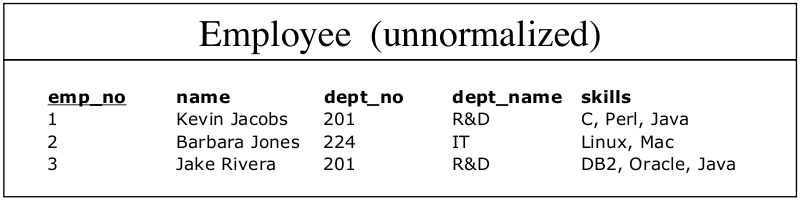
\includegraphics[scale=0.4]{unnormalized.png} 
	\item[First Normal Form (1NF)] \underline{all table entries (attribute values) are atomic} \\
	no repeating columns (attributes) within a row, no multi-valued columns \\
	queries and sorting become easier \\
	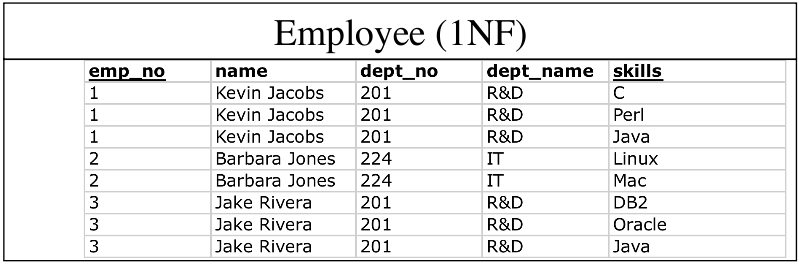
\includegraphics[scale=0.4]{1NF.png} 
	\item[Second Normal Form (2NF)]Functional Dependence: \underline{all attributes functionally depend on primary key}: non-depending stuff $\to$ new table\\
	prevents insert/deletion anomalies \\
	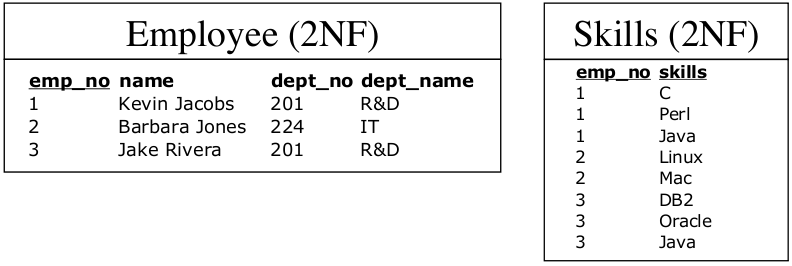
\includegraphics[scale=0.4]{2NF.png} 
	\item[Third Normal Form (3NF)] standard relational form for use\\
	every FD $A_1,\dots.A_n\to B$ satisfies at least one of:
	\begin{itemize}
		\item the FD is trivial
		\item the FD follows from a key, because $\{A_1,\dots,A_n\}$ or subset of it is already a key of $R$
		\item $B$ is a key attribute (element of a key of $R$)
	\end{itemize}
	or: \underline{remove transistive dependence} {\tiny something is not dependent in the key} into subtables\\
	prevents update anomalies\\
	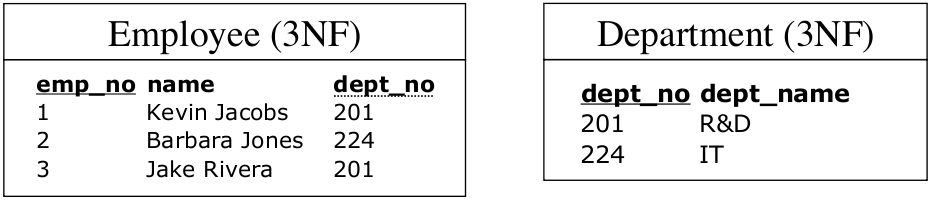
\includegraphics[scale=0.4]{3NF.png}
	\item[Determinante:] Attributmenge, von der andere Attribute funktional abhängen
	\item[Schlüsselkandidat:] Menge von Attributen, von der alle Attribute der Relation voll funktional abhängig sind.
	\item[Boyce Codd Normal Form (BCNF)] more restrictive than 3NF, easier to define, short: "`all FDs are already enforced (represented) by keys"'\\
	anders: BCNF ist erfüllt, wenn (3NF gilt,) \underline{jede Determinante Schlüsselkandidat} (oder die Abhängigkeit trivial) ist. 
	\item[Fourth Normal Form (4NF)] nur triviale Mehrwertige Abhängigkeiten enthalten, oder die MwA gehen von Superschlüsseln aus. \\
	kurz: Es darf nicht etwa $n$-mal Attribut $a$ und unabhängig davon $m$-mal Attribut $b$ vom Schlüsselwert abhängen.\\
	in 4NF überführen: jede MwA in extra Tabelle auslagern
	\item[decomposition:] If $R$ is not in BCNF, split it into two tables along the violating FD: \\
	If $A\to B$ violates BCNF remove B from $R$ and add new relation (table) $A\to B$
	\item[lossless decomposition:] if the intersection of the attributes of the new tables is a key of at least on of them \\
	the original relation can be reconstructed via a natural join
	\item[Normalisation]
	\item[minimal cover:] want a minimal cover, $\mathcal{F}'$ with same transitive closure $(\mathcal{F}')^+=\mathcal{F}^+$
	\begin{itemize}
		\item Canonicalize rhs: Replace FD $\alpha\to B_1,\dots,B_m$ by corresponding set of FDs: $\alpha\to B_i,1\leq i\leq m$
		\item Minimize lhs: For each FD $A_1,\dots,A_n\to B$ and each $i=1,\dots,n$ check, if $B\in\{A_1,\dots,A_{i-1},A_{i+1},\dots,A_n\}^+_\mathcal{F}$, if so $\mathcal{F}\leftarrow(\mathcal{F}-\{A_1,\dots,A_n\to B\})\cup\{A_1,\dots,A_{i-1},A_{i+1},\dots,A_n\to B\}$
		\item Remove implied FDs: For each FD $\alpha\to B$, check if $B\in\alpha^+_{\mathcal{F}-\{\alpha\to B\}}$, if so: $\mathcal{F}\leftarrow \mathcal{F}-\{\alpha\to B\}$
	\end{itemize}
	\item[3NF synthesis algorithm] produces lossless decomposition into 3NF and preserves FDs
	\begin{itemize}
		\item Compute minimal cover of given FDs $\mathcal{F}'$
		\item For each lhs in $\mathcal{F}'$ create relation with attributes: $\mathcal{A}=\alpha\cup\{ B\vert\alpha\to B\in\mathcal{F}' \}$
		\item if none of these relations contain a a key of original relation $R$ add one relation containing the attributes of a key of $R$
		\item For any two relations $R_{1,2}$ constructed, if the schema of $R_1$ is contained in $R_2$ drop $R_1$
	\end{itemize}
	\item a "`good"' ER will result in a high normal form
\end{description}

\end{document}
